\documentclass[12pt]{article}
\usepackage{amsmath}
\usepackage{tikz}
\begin{document}
\title{Computer Science 181, Homework 5}
\date{May 4th, 2018}
\author{Michael Wu\\UID: 404751542}
\maketitle

\section*{Problem 1}

Assume for contradiction that \(\bar{L}\) is a finite state language. Then by the closure properties of finite state languages,
its complement \(L\) is a finite state language. Then by the pumping lemma there exists some \(p\) such that whenever a string \(s\in L\)
is longer than \(p\), it can be split into three strings \(s=xyz\) such that \(|y|\geq 1\), \(|xy|\leq p\), and \(xy^nz\in L\) for any integer \(n\geq 0\).
Consider the string \(s\in L\), where \(s=ww\) and \(|w|>p\). Let \(w\) be a string beginning with \(a\) followed entirely by \(b\)'s.
Because \(|xy|\leq p\), the leftmost \(w\) must contain \(x\) and \(y\). If \(y\) consists of only \(b\)'s then \(xy^nz\notin L\) for \(n=2\),
since this would mean that \(xy^2z\) has the form \(ab^{k_1}ab^{k_2}\), where \(k_1>k_2\). Strings of this format are not in \(L\). If \(y\) contains an \(a\), then
it can only contain a single \(a\). So \(xy^2z\) will have three \(a\)'s, since there are two in \(xyz\) and one in \(y\). Then \(xy^2z\notin L\), since \(L\) must
contain an even number of both \(a\)'s and \(b\)'s. This is a contradiction, since the pumping lemma says that \(xy^nz\in L\) for all \(n\geq 0\). Thus our assumption
that \(\bar{L}\) is a finite state language cannot be correct, and \(\bar{L}\) is a non finite state language.

\section*{Problem 2}

Yes it is ambiguous. The string
\begin{center}
\begin{verbatim}
atom+atom+atom
\end{verbatim}
\end{center}
can be parsed as either
\begin{center}
        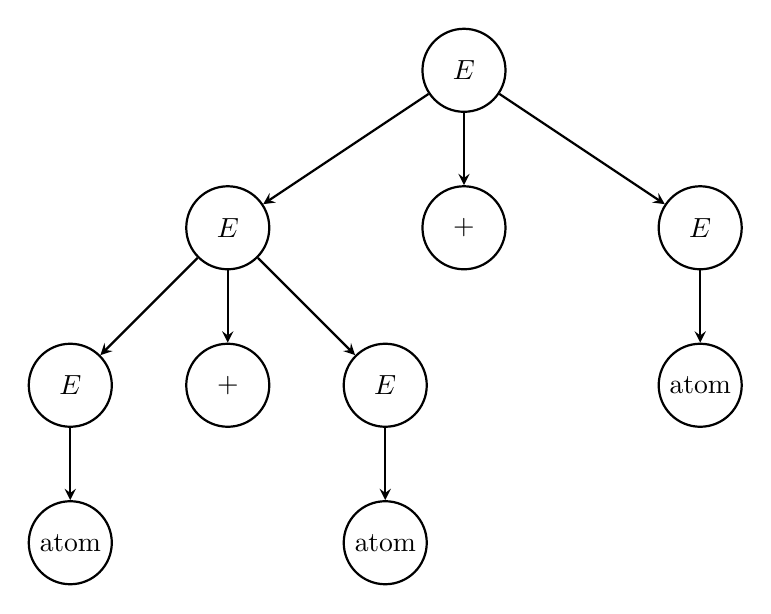
\begin{tikzpicture}
                \begin{scope}[auto, every node/.style={thick, draw,circle,minimum size=3em,inner sep=1}]
                        \node (E1) at (0,0) {\(E\)};
                        \node (E2) at (-3,-2) {\(E\)};
                        \node (E3) at (3,-2) {\(E\)};
                        \node (E4) at (-5,-4) {\(E\)};
                        \node (E5) at (-1,-4) {\(E\)};

                        \node (P1) at (0,-2) {\(+\)};
                        \node (P2) at (-3,-4) {\(+\)};
                        \node (A1) at (3,-4) {atom};
                        \node (A2) at (-5,-6) {atom};
                        \node (A3) at (-1,-6) {atom};
                \end{scope}
                \begin{scope}[auto, every node/.style={minimum size=1em,inner sep=1}, every path/.style={thick, ->, >=stealth}]
                        \path (E1) edge (E2);
                        \path (E1) edge (E3);
                        \path (E1) edge (P1);

                        \path (E2) edge (E4);
                        \path (E2) edge (E5);
                        \path (E2) edge (P2);
                        \path (E3) edge (A1);
                        \path (E4) edge (A2);
                        \path (E5) edge (A3);
                \end{scope}
        \end{tikzpicture}
\end{center}
or it can be parsed as
\begin{center}
        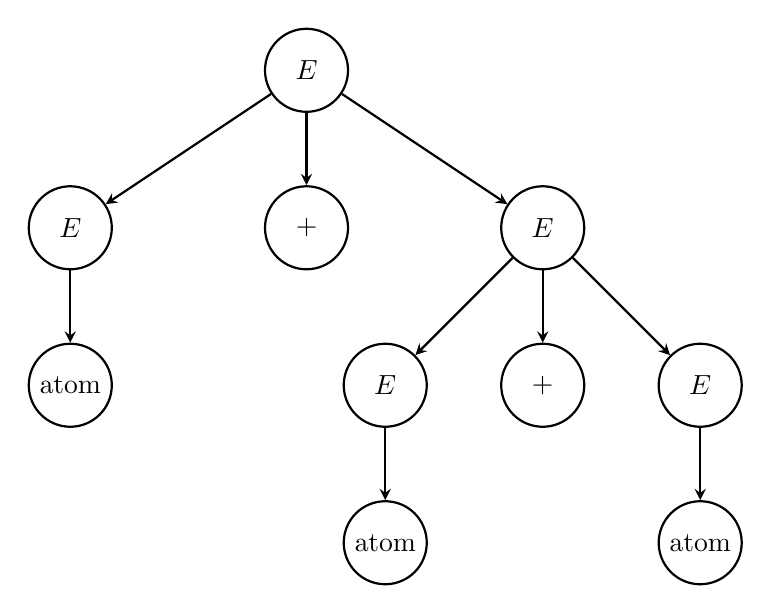
\begin{tikzpicture}
                \begin{scope}[auto, every node/.style={thick, draw,circle,minimum size=3em,inner sep=1}]
                        \node (E1) at (0,0) {\(E\)};
                        \node (E2) at (3,-2) {\(E\)};
                        \node (E3) at (-3,-2) {\(E\)};
                        \node (E4) at (5,-4) {\(E\)};
                        \node (E5) at (1,-4) {\(E\)};

                        \node (P1) at (0,-2) {\(+\)};
                        \node (P2) at (3,-4) {\(+\)};
                        \node (A1) at (-3,-4) {atom};
                        \node (A2) at (5,-6) {atom};
                        \node (A3) at (1,-6) {atom};
                \end{scope}
                \begin{scope}[auto, every node/.style={minimum size=1em,inner sep=1}, every path/.style={thick, ->, >=stealth}]
                        \path (E1) edge (E2);
                        \path (E1) edge (E3);
                        \path (E1) edge (P1);

                        \path (E2) edge (E4);
                        \path (E2) edge (E5);
                        \path (E2) edge (P2);
                        \path (E3) edge (A1);
                        \path (E4) edge (A2);
                        \path (E5) edge (A3);
                \end{scope}
        \end{tikzpicture}
\end{center}

\section*{Problem 3}

\begin{align*}
        L_{ists}&=(V,\Sigma,R,S)\\
        V&=\{A,B\}\\
        R&=\{A\rightarrow \text{atom} \mid \text{(}B\text{)},\\
        &\hphantom{==}B\rightarrow A \mid BB \mid \epsilon\}\\
        S&=A
\end{align*}

\end{document}
